\section{Introduction}\label{section:Intro}

The Large Underground Xenon (LUX) experiment recently published a search for direct evidence of Weakly Interacting Massive Particles (WIMPs)~\ref{Run4Paper}.  The search was performed with a dual-phase (liquid and gas) xenon time projection chamber (TPC) containing 250 kg of liquid xenon in the active detector volume.  Recoil events were observed as prompt VUV photons from scintillation (S1), and as liberated electrons which were drifted to the liquid surface via an applied electric field (S2). 


As with all dual-phase TPCs, the S1 and S2 signals varied according to the vertex position of the interaction.  These signal variations resulted from both detector inefficiencies and field induced effects.  In the case of detector inefficiencies, the detection efficiency of S1 photons was roughly 30\% larger for events close to the cathode, when compared to those at the liquid surface. Similarly, loss of electrons to electronegativity impurities resulted in depth-dependent variation in the S2 signal, with 20-50\% of electrons liberated at the bottom of the detector reaching the liquid surface, depending on the purity of the liquid xenon at the time.  These sources of pulse area variations are independent of the energy of an event, or the type of recoil interaction that occurred, and can therefore be removed by applying event-agnostic position dependent signal corrections as was done in~\ref{Run3Reanalysis}.  Note that these energy and recoil-independent signal variations will be referred to as "detector inefficiencies" throughout this paper. 


As detailed in~\ref{Run4Paper}, the anode, gate, and cathode grids underwent a conditioning campaign inbetween LUX's WS2013 and WS2014–16 data collections.  This campaign increased the operating extraction field from 2.9 kV/cm to 3.5 kV/cm, and the detector's electron extraction efficiency from 49$\pm$3\% to 73$\pm$4\%.  After completing the grid conditioning campaign, deviations in the trajectory of free electrons, as well as inconsistencies in electron lifetime measurements across multiple sources, led to the conclusion that a non-uniform and time-varying negative
charge density in the polytetrafluoroethylene (PTFE)
panels had developed during the campaign.

The resulting nonuniform drift field introduced a second source of position dependent signal variations.  During a recoil event, ionizing radiation produces both ionization and excitation of the xenon atoms.  The xenon excimers (Xe$_2^*$) produce scintillation light as they return to the ground state, which we observe as our S1 signal. Some of the electrons produced during ionization escape the location of the event, drift to the top of our detector, and produce our S2 signal.  The electrons that do not escape the event recombine with the ionized xenon atoms in a process called recombination, producing additional xenon excimers that contribute to the S1 signal.  Recoil events which occur in a lower field region of the detector have a higher chance to recombine, and therefore produce more S1 signal and less S2 signal than an equivalent event in a high field region.  The strength of this effect is dependent on the energy of the event and whether the event is an electron recoil (ER) or a nuclear recoil (NR) (Figure \ref{fig:LYQY}).  Note that these energy and recoil-dependent signal variations will be referred to as "field effects" in this paper.  

\begin{center}
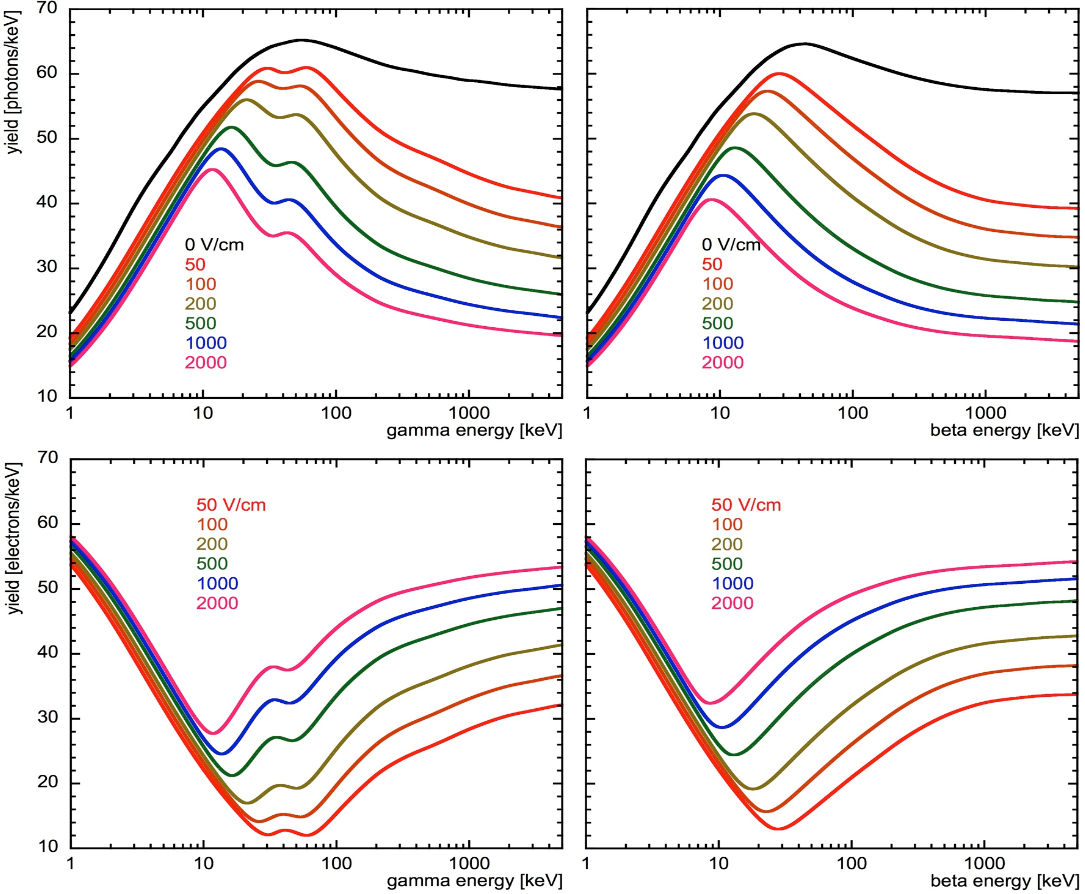
\includegraphics[scale=0.25]{Run04Corrections/Recomb.png}
\captionof{figure}{Predictions from NEST for the light yield (top row) and charge yield (bottom row) of electron recoil event from gamma ray interaction (left column) and beta particle interaction (right column).  Field values are indicated by the colored lines.  Light yield and charge yield have less dependence on the field strength for lower energy events.  \cite{RecombSource} }
 \label{fig:LYQY}
\end{center}
